\documentclass{article}
\usepackage[margin=1.5cm,bottom=2cm]{geometry}
\usepackage{fancyhdr}
\usepackage{graphicx}
\pagestyle{fancy}

\begin{document}
\fancyhead[L]{ 
\includegraphics[width=2cm]{au_logo.png} }
\fancyhead[R]{PHYS 4220: Computational Physics}
\fancyfoot[C]{\thepage}
\vspace*{0cm}
\begin{center}
	{\LARGE \textbf{Homework 0}}\\
	\vspace{0.25cm}
	{\Large Due: Friday, September 4}
\end{center}

\begin{enumerate}
	\item Create random vector of size 10 and replace the maximum value by 0.
	\item Write a function which converts a 3 dimensional vector from Cartesian to spherical coordinates. Write the reverse function, which converts a spherical vector to Cartesian coordinates.
	\item\label{problem:block_sum} Given a 16x16 array of numbers, write a function which computes the 4x4 block sum array where each element corresponds to the sum of a 4x4 sub-array of the input array (see Figure \ref{block_sum}). Plot the resulting array.
	\begin{figure}[ht!]
		\centering
		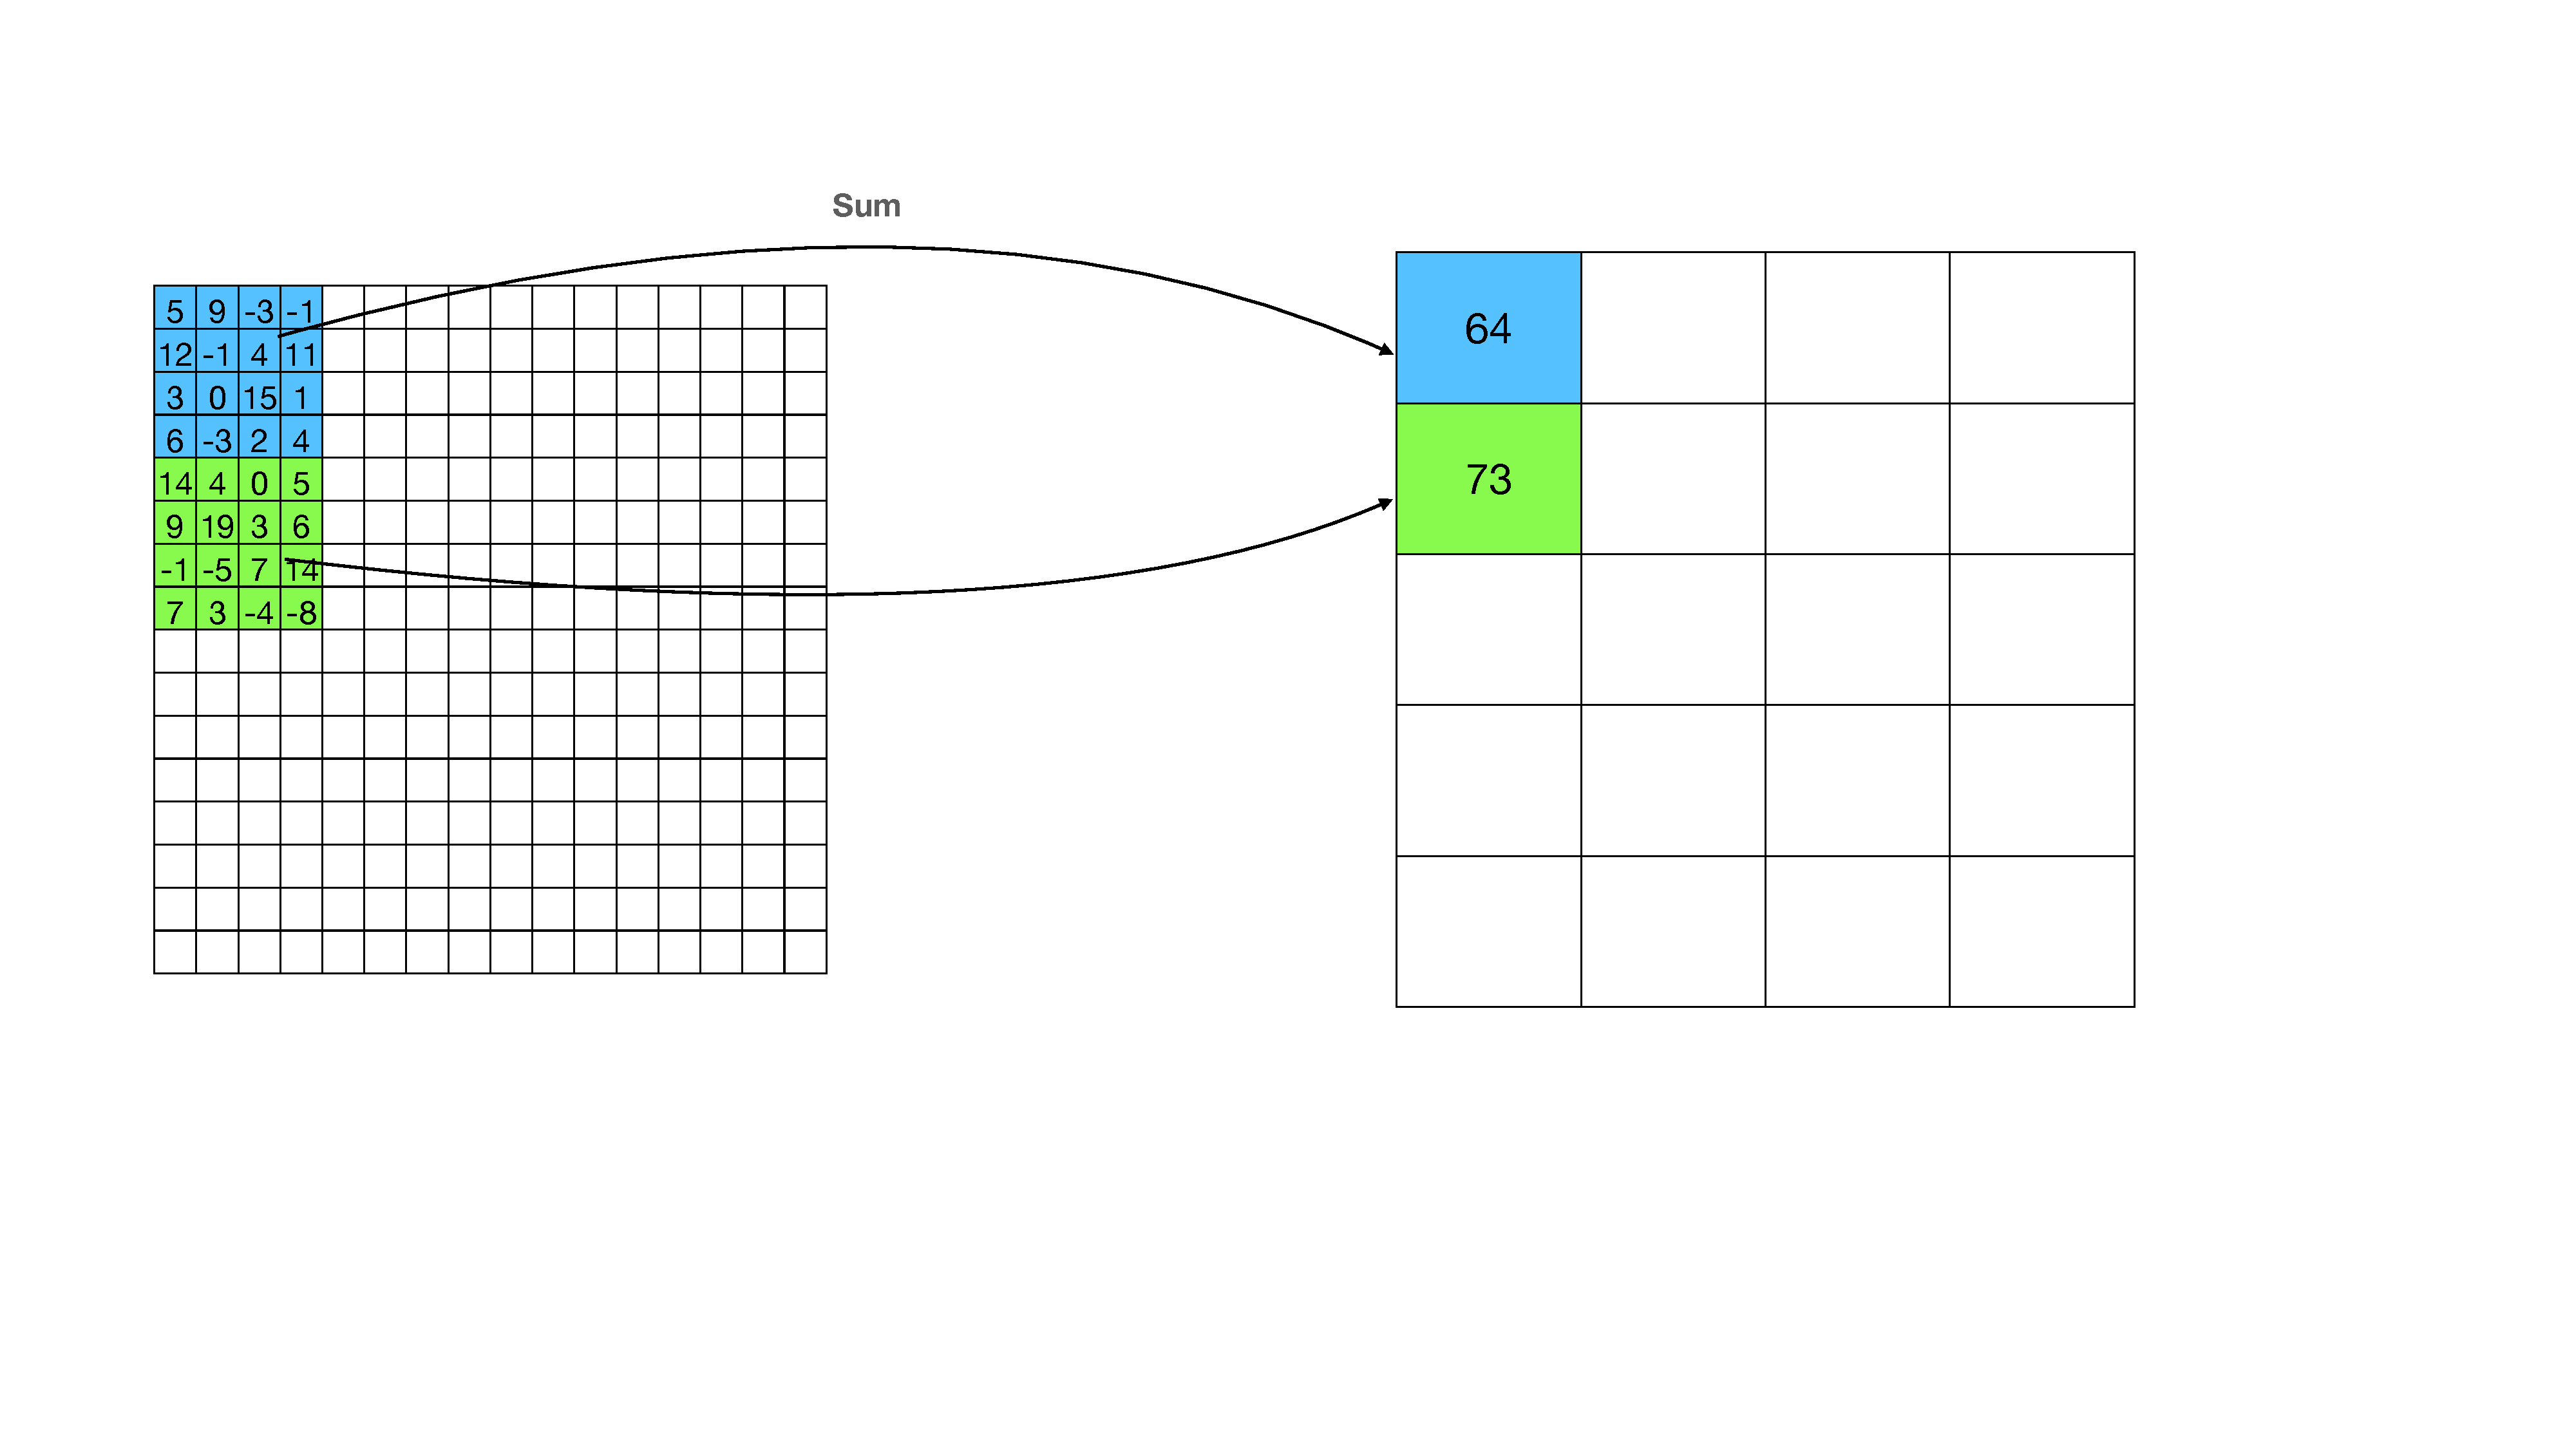
\includegraphics[width=0.6\textwidth]{block_sum}
		\caption{Figure for problem \ref{problem:block_sum}}
		\label{block_sum}
	\end{figure}

	\item Generate a random (uniform) set of 2D points $<x,y>$. Make a plot of the distribution of $r=\sqrt{x^2+y^2}$. Do the same for 3D and 4D points, where $r=\sqrt{\sum_{i=0}^D r_i^2}$
	
	\item\label{problem:mcpi} We can use a random generator to approximate pi. This exercise will walk you through how to do this. 
	\begin{enumerate}
		\item Draw a large number of random 2D points $<x,y>$ from a uniform distribution over a fixed area. 
		\item Calculate the fraction of all generated points which ``land'' inside a circle of given radius $R$ (see Figure \ref{mcpi}). The area of the circle is then equal to the area over which the points were generated multiplied by the fraction of points landing within the circle.
		\item What is the ratio of your calculated area to $R^2$?
		\item Make a plot of this ratio as a function of number of generated points (should contain at least 10 points)
	\end{enumerate}
	
		\begin{figure}[ht!]
		\centering
		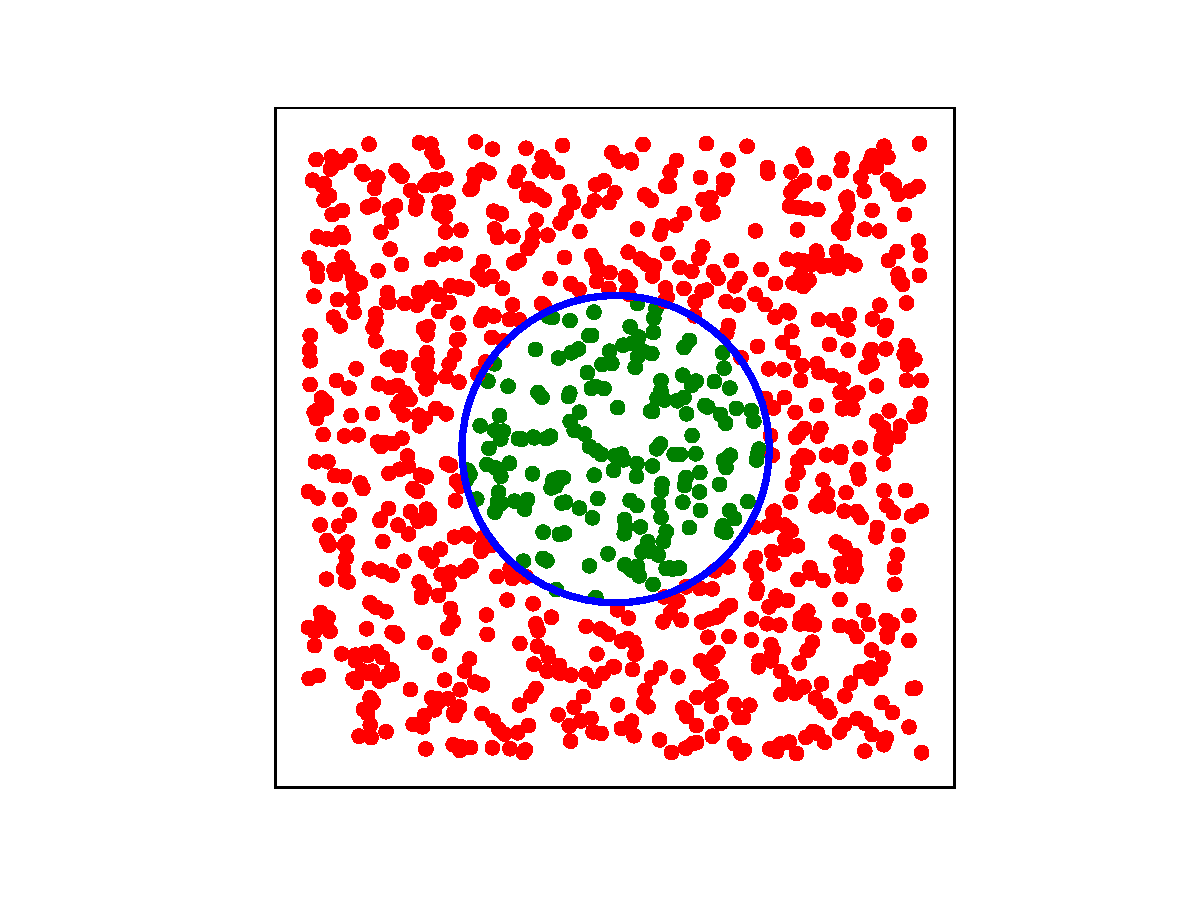
\includegraphics[width=0.45\textwidth]{mc_pi}
		\caption{Figure for problem \ref{problem:mcpi}}
		\label{mcpi}
	\end{figure}

\newpage
\item A mass $m$ hangs vertically at the end of a spring with spring constant $k$.  Write and normalize the differential equation for the displacement of the mass $x(t)$ from equilibrium as a function of time. Assume $x(0)=0$,$\frac{dx}{dt}(0) = v_0$. Neglect frictional forces.

\item A stationary ball of mass $m$ is released a distance $X_0$ from the surface of the Earth. Write and normalize the differential equation of motion for the position of the ball as it falls due to gravity. Neglect frictional forces.
\end{enumerate}

\end{document}